\section{Motivation architecture}
\label{sec:motivation-architecture}

	%	TODO: rewrite 
	This section presents the motivation and goal structure of the Standardisation Unit. This will help determine the scope and rationale for the current architecture specification. The analysis of the motivation structure was not conducted in depth in order to constitute a decision making tool for the management but rather was aimed at accounting for the context of the publishing workflow which is the final goal of this architecture.
	
	Nonetheless, this motivation view helps address the questions why a demand is meaningful, model crucial drivers and root causes behind the demand, actual goals and related outcomes, as well as concrete requirements for further development. In short it answers the questions to WHOM, WHY and WHAT.
	
	\subsection{Overall motivation structure}
	\label{sec:how-to-motivation}		
	
	The structure of motivations, in ArchiMate, is hierarchically organised in several layers. For simplicity, we have chosen to use the top four layers: \textit{stakeholders, drivers, assessments and goals}; leaving out the \textit{outcomes}, \textit{principles} and \textit{requirements}. \mbox{Figure \ref{fig:morivation-structure}} depicts the organisation of the motivation architecture. The structure starts at the top with enumerating the stakeholders, who are individuals, teams or organisations that represent their interests in the effects of \mbox{the architecture \citep{archimate3.1}}. 
	
	\begin{figure}[h]
		\centering
		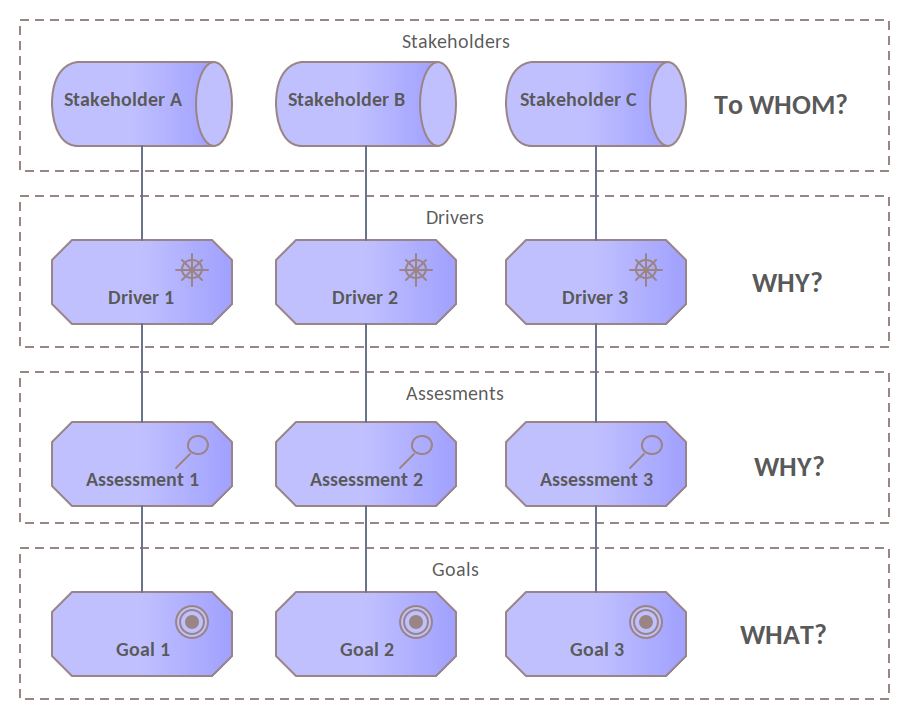
\includegraphics[width=0.7\textwidth]{images/views/Motivation view.png}
		\caption{The layered motivation structure}
		\label{fig:morivation-structure}
	\end{figure}
	
	Stakeholders have associated interests, concerns or drivers, which represent internal or external conditions that motivate an organisation to define goals \citep{archimate3.1}.
	
	
	%	\begin{wrapfigure}{r}{0.65\textwidth}
	%		\centering
	%		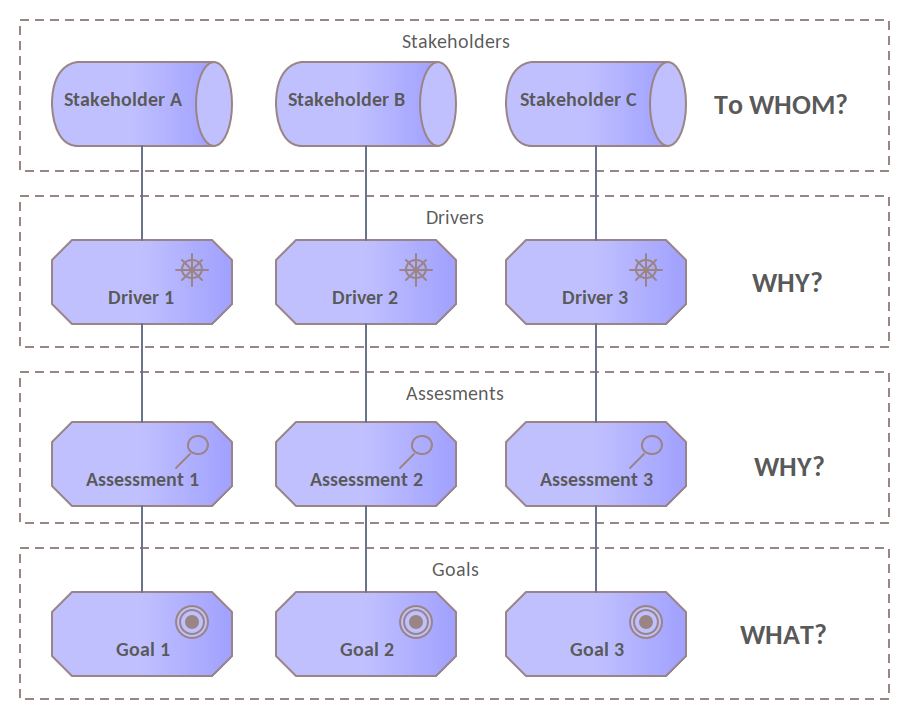
\includegraphics[width=0.67\textwidth]{images/views/Motivation view.png}
	%		\caption{The layered motivation structure}
	%	\end{wrapfigure}
	 
	Assessments represent results of analysis of the state of affairs with respect to some driver. They reveal strengths and weaknesses, opportunities or threats to an area of interest \citep{archimate3.1}.
	
	Assessments are associated with goals, which represent a high level statement of intent, direction to desired end state for an organisation and its stakeholders \citep{archimate3.1}. 
	
	Next we present the SU motivation structure spread over several sections.
	
	\subsection{Stakeholders and their roles}
	
	The Standardisation Unit involves multiple stakeholders. We can enumerate them but the list will be long and outside the scope of this exercise. Instead, we highlight the most important ones and in addition we group them based on the role they play in interaction with SU. In Figure \ref{fig:stakehodlers-roles} the roles are depicted as aggregate stakeholders in a grouping frame in the middle of the figure. Above the roles are placed the most important external stakeholders while below are enumerated the stakeholders from the PO.
	
	\begin{figure}[hbt!]
		\centering
		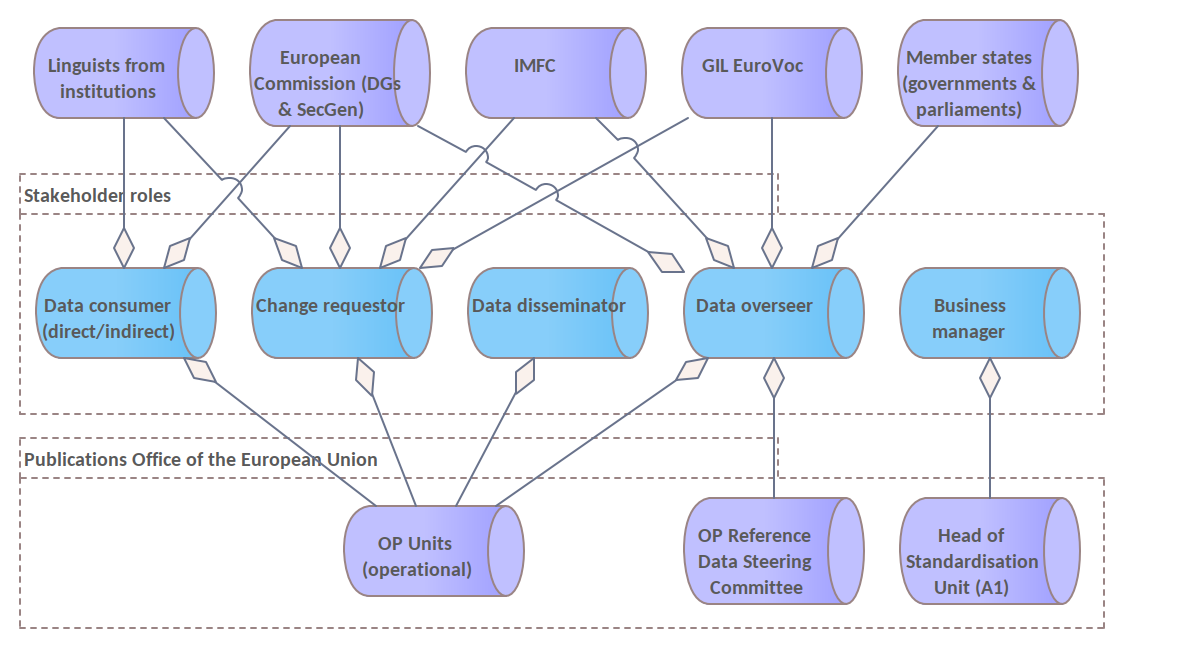
\includegraphics[width=0.8\textwidth]{images/motivation/Stakeholders & Roles.png}
		\caption{The layered motivation structure}
		\label{fig:stakehodlers-roles}
	\end{figure}
	
	The most important external stakeholders are: European Commission together with the Secretary General and all of the Commission’s Directorates, the Inter-institutional Metadata and Formats committee (IMFC), the EuroVoc Committee (Group interinstitutional Lex (GIL)-subgroup EuroVoc), EU member states represented by their governments and parliaments, and Linguists from different institutions and with a particular interest to the IATE project.
	 
	In the Figure \ref{fig:stakehodlers-roles} the OP stakeholders are placed in organisation bounding context, as the SU is a part of the PO and so its sibling units are not entirely external but members of the same organisation. The stakeholders within PO are the various units that use the reference data (e.g. Cellar team, OP Portal team, EurLex team, and others). A Reference Data Steering Committee is planned to be formed in the near future in order to coordinate and harmonise the published reference data. And finally the Head of Standardisation Unit who is in charge of running the enterprise.
	 
	In order to easier account for the stakeholders drivers, interests and goals, we grouped them based on their roles in interaction with SU. In Figure (above) the roles are depicted as aggregate stakeholders in a grouping frame in the middle of the figure. The roles are: data consumers, data requestors, data disseminators, data overseers and business managers. Next we describe each of the roles and then briefly enumerate the stakeholders.
	 
	The \textit{consumers} of assets are the users that directly engage with the published assets (direct consumer) or the users of applications and services that are making use of the published assets (indirect consumer).
	
	The \textit{change requesters} are the agents that need and therefore requires particular content to be available as reference data. 
	
	The \textit{data disseminators} are services and platforms where the reference assets are published for broad public consumption.
	
	The \textit{data overseers} are the agents that ensure that the content satisfies business needs is harmonised, coherent and complete. It is also responsible for the content correctness and harmonization among multiple stakeholders and its usefulness in broader context of application. Usually the role of data overseers is played by the standardization committees, steering committees and data stewards at large.
	
	\subsection{Drivers: primary}
	
	We have identified four \textit{primary drivers}, three \textit{secondary drivers} and two \textit{internal efficiency drivers}. The distinction between primary and secondary drivers is based on whether the driver is shared between the external and internal stakeholders (in this case the business management).
	Figure \ref{fig:primary-drivers} depicts the main stakeholders and their concerns, where the business manager, in this case head of the SU, has the same primary concerns as the main stakeholder roles.
	
	\begin{figure}[hbt!]
		\centering
		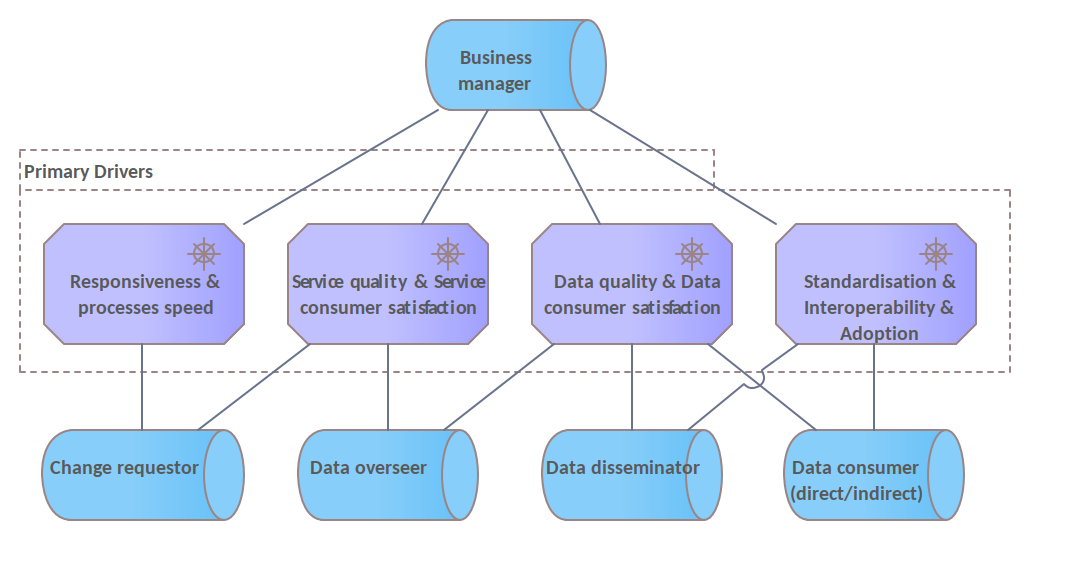
\includegraphics[width=0.9\textwidth]{images/motivation/Primary drivers.png}
		\caption{Primary drivers, motivating both, the internal and external stakeholders}
		\label{fig:primary-drivers}
	\end{figure}
	
	For change requesters, the interaction \textit{responsiveness and the speed of the asset lifecycle process} is of primary concern. The sooner the requests are processed and analysed the sooner they can be implemented, processed and published. The goal of the SU is to reach the swiftness of publishing overnight change requests, as compared to the current situation when four major publications are scheduled per year allowing also a few urgent ones in between.
	
	The \textit{quality of service} provided by the SU at large and the service consumer satisfaction is a direct concern for the change requesters and data overseers as primary users various SU services. 
	
	The \textit{quality of data} is of special interest for the data overseers as they are directly responsible for this aspect and implicitly of the data consumer satisfaction. The data quality here has a wide meaning covering aspects of formal, semantic and conceptual correctness while also being timely and up to date with the business. Besides the data overseers, the data users are also interested in high quality reference data. The data disseminators are indirectly affected by the quality of the data they distribute and share this interest to a lesser degree. 
	
	The last of the primary drivers is the \textit{standardisation, interoperability and adoption}, which is a major concern for the data disseminators and the data users. This driver covers the adoption of widely used meta-models, formally well defined models representing shared conceptualisation of major bodies and organisations, usage and implementation of national and international standards proposed by the standardisation bodies (e.g. ISO, W3C, OMG). These standards refer not only to aspects of data representation, but also to protocols, exchange schemas, validation mechanisms and other tools facilitating systemic interoperability. 
	
	\subsection{Drivers: secondary}
	The secondary drivers are those that are important to either external stakeholders ro the internal ones alone.
	
	\begin{figure}[h!]
		\centering
		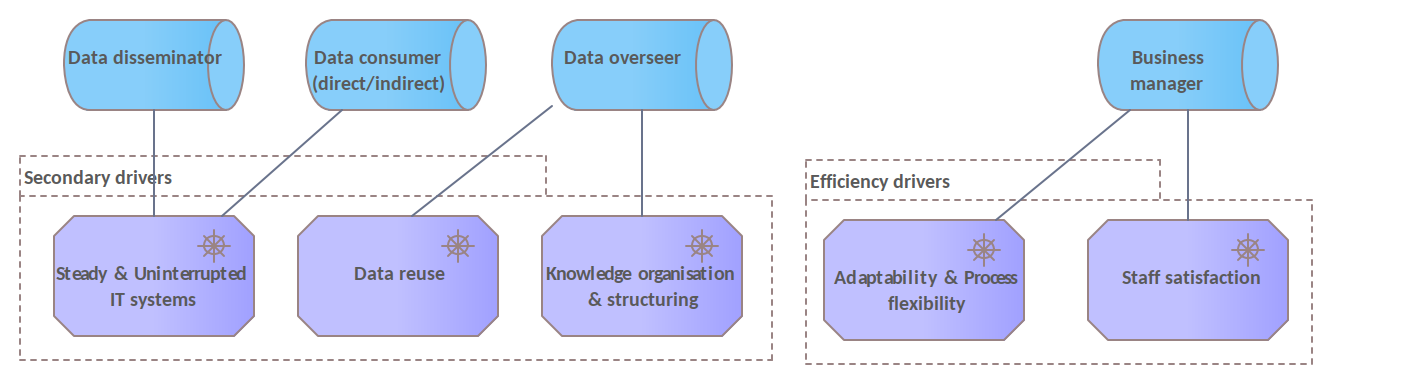
\includegraphics[width=1.05\textwidth]{images/motivation/Secondary drivers.png}
		\caption{Secondary drivers, motivating either internal or external stakeholders}
		\label{fig:secondary drivers}
	\end{figure}

	%	TODO: describe
	
	\subsection{Assessment: Responsiveness and processing speed}
	
	\begin{figure}[h]
		\centering
		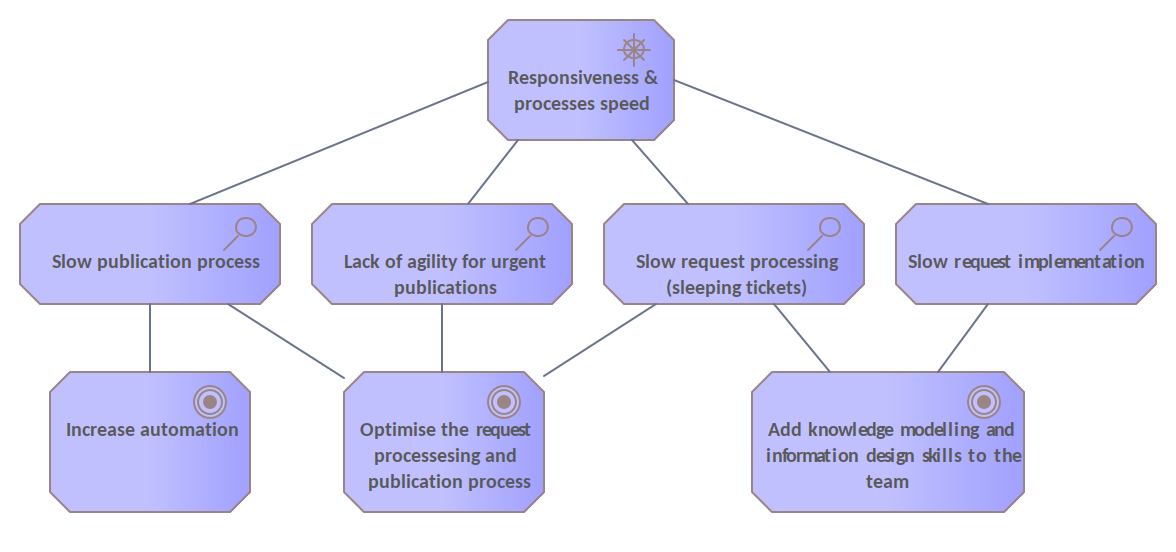
\includegraphics[width=\textwidth]{images/motivation/Responsiveless & Process Speed.png}
		\caption{The assessment of the responsiveness and processing speed driver}
		\label{fig:responsiveness-and-processing-speed}
	\end{figure}

	\subsection{Assessment: Data quality}

	\begin{figure}[h]
		\centering
		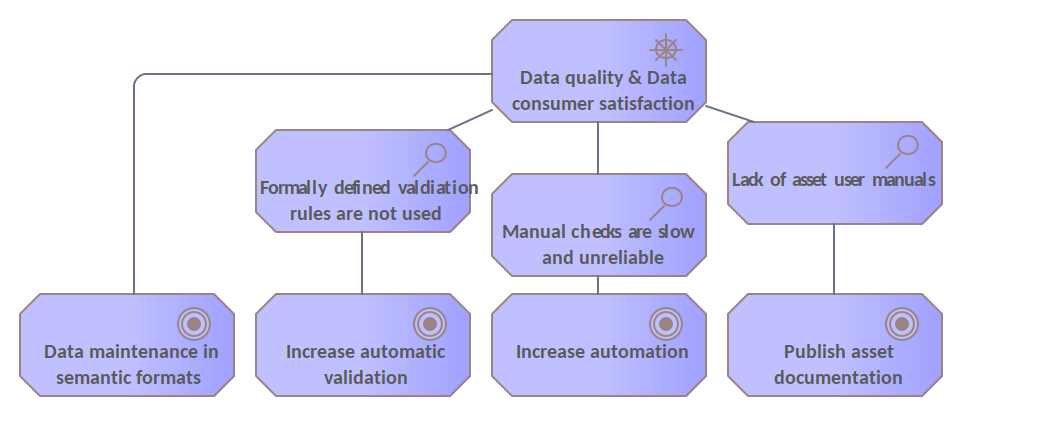
\includegraphics[width=0.9\textwidth]{images/motivation/Data quality.png}
		\caption{The assessment of data quality and data consumer satisfaction}
		\label{fig:data-quality}
	\end{figure}

	\subsection{Assessment: Service quality}

	\begin{figure}[h]
		\centering
		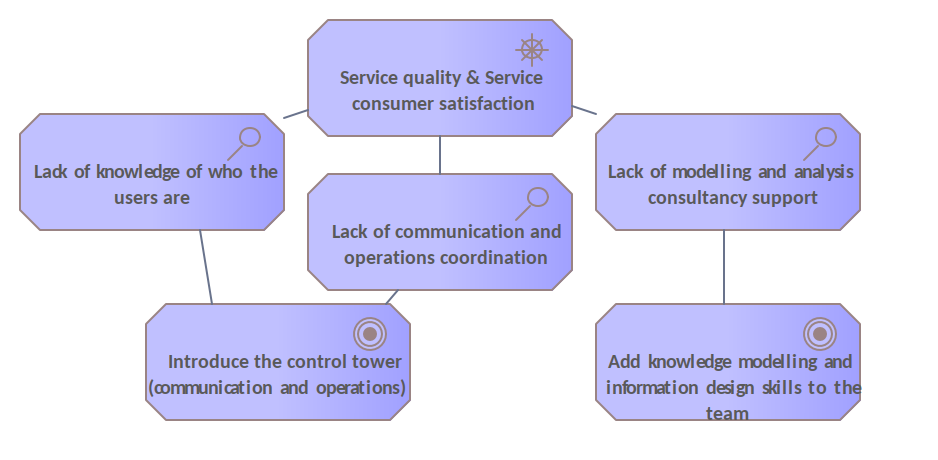
\includegraphics[width=0.8\textwidth]{images/motivation/Service quality.png}
		\caption{The assessment of service quality and service consumer satisfaction}
		\label{fig:service-quality}
	\end{figure}